%!TEX program = Xelatex
\documentclass{article}
%\usepackage{ctex}
\usepackage{amsmath,amscd,amsbsy,amssymb,latexsym,url,bm,amsthm}
\usepackage{epsfig,graphicx,subfigure}
\usepackage{enumitem,balance,mathtools}
\usepackage{wrapfig}
\usepackage{booktabs}
\usepackage{threeparttable}
\usepackage{mathrsfs, euscript}
\usepackage[usenames]{xcolor}
\usepackage{hyperref}
\usepackage{caption}
%\usepackage{subcaption}
\usepackage{float}
\usepackage{listings}
\usepackage{tabularx}
%\usepackage{enumerate}
%\usepackage{algorithm}
%\usepackage{algorithmic}
%\usepackage[vlined,ruled,commentsnumbered,linesnumbered]{algorithm2e}
\usepackage{algorithm}  
\usepackage{algorithmicx}  
\usepackage{algpseudocode}
\usepackage{tikz}
\usetikzlibrary{arrows,shapes,chains}
\usetikzlibrary{positioning}

\newtheorem{theorem}{Theorem}[section]
\newtheorem{lemma}[theorem]{Lemma}
\newtheorem{proposition}[theorem]{Proposition}
\newtheorem{corollary}[theorem]{Corollary}
\newtheorem{exercise}{Exercise}[section]
\newtheorem*{solution}{Solution}

\renewcommand{\thefootnote}{\fnsymbol{footnote}}

\newcommand{\postscript}[2]
    {\setlength{\epsfxsize}{#2\hsize}
    \centerline{\epsfbox{#1}}}

\renewcommand{\baselinestretch}{1.0}

\setlength{\oddsidemargin}{-0.365in}
\setlength{\evensidemargin}{-0.365in}
\setlength{\topmargin}{-0.3in}
\setlength{\headheight}{0in}
\setlength{\headsep}{0in}
\setlength{\textheight}{10.1in}
\setlength{\textwidth}{7in}

\title{Sudoku Recognizer And Solver\\EI339 Programming Project}
\author{Liu Yanming StudentID:518030910393}

\begin{document}

\maketitle

\section{The Jobs I Have Done}
\begin{enumerate}
    \item Run the code in ``OpenCV Sudoku Solver and OCR'' successfully, and understand the code structure and principle.
    \item Read LeCun's paper and implement a simple network like LeNet-5, and then implement a rough RSNet-18 to learn about more modern method and get better recognition effect.
    \item Train both network above on the data set MNIST and EI339-CN (data set for Chinese hand-written number, made by the classmates). And get the desired accuracy on the test set.
    \item Implement a Sudoku puzzle solver using a CSP algorithm called dancing links.
    \item Using the test example to evaluate the model. Completely debug and test all the processes of recognition and solving, though the result is not satisfactory.
\end{enumerate}
Next, I will introduce the above parts in detail based on my understanding.

\section{The ``OpenCV Sudoku Solver and OCR'' Lib}
The processes of the programming given in this library:
\begin{figure}[htb]
\centering
\includegraphics[width=0.5\linewidth]{./processes.png}
\end{figure}~\\
The running result:
\begin{figure}[htb]
\centering
\includegraphics[width=0.5\linewidth]{./lib_result.png}
\end{figure}

\section{CNN Network Model}
\subsection{A Simple Network Similar To LeNet-5}
The structure of the network I used:
\begin{figure}[htb]
\centering
\begin{minipage}[h]{0.48\linewidth}
\begin{figure}[H]
\centering
\begin{tikzpicture}[node distance=0.25cm, scale=0.75]
\tikzstyle{feature} = [trapezium, draw = black]
\tikzstyle{conv} = [rectangle, draw = black]
\tikzstyle{pool} = [rectangle, draw = black]
\node (input) [feature] {$1 \times 28 \times 28$};
\node (conv1) [conv, below = of input] {conv $1\times 6\times 5\times 5$, padding=2};
\node (p1) [pool, below = of conv1] {max pool $2\times 2$};
\node (f1) [feature, below = of p1] {$6\times 14 \times 14$};
\node (conv2) [conv, below = of f1] {conv $6\times 16\times 5\times 5$};
\node (p2) [pool, below = of conv2] {max pool $2\times 2$};
\node (f2) [feature, below = of p2] {$16\times 5\times 5$};
\draw [->] (input) -- (conv1);
\draw [->] (conv1) -- (p1);
\draw [->] (p1) -- (f1);
\draw [->] (f1) -- (conv2);
\draw [->] (conv2) -- (p2);
\draw [->] (p2) -- (f2);  
\node (fc1) [conv, below = of f2] {fc $400\times 120$};
\node (fc2) [conv, below = of fc1] {fc $120 \times 84$};
\node (fc3) [conv, below = of fc2] {fc $84\times 18$};
\node (out) [feature, below = of fc3] {output $18$-dim};
\draw [->] (f2) -- (fc1);
\draw [->] (fc1) -- (fc2);
\draw [->] (fc2) -- (fc3);
\draw [->] (fc3) -- (out);
\end{tikzpicture}
\caption{LeNet-5 like structure}
\label{lenet5}
\end{figure}
\end{minipage}
\begin{minipage}[h]{0.48\linewidth}
\begin{figure}[H]
\centering 
\begin{tikzpicture}[node distance=0.35cm, scale=0.75]
\tikzstyle{myshape} = [rectangle, draw = black]
\node (in) [myshape] {in};
\node (conv) [myshape, below = of in] {conv};
\node (batchnorm) [myshape, below = of conv] {batchnorm};
\node (relu) [myshape, below = of batchnorm] {relu};
\node (pool) [myshape, below = of relu] {pool};
\node (out) [myshape, below = of pool] {out};
\draw [->] (conv) -- (batchnorm);
\draw [->] (batchnorm) -- (relu);
\draw [->] (relu) -- (pool);
\draw [->] (in) -- (conv);
\draw [->] (pool) -- (out);
\end{tikzpicture}
\caption{The detailed structure of the convolution layer}
\label{convlayer}
\end{figure}
\begin{figure}[H]
\centering
\begin{tikzpicture}[node distance=0.35cm, scale=0.75]
\tikzstyle{conv} = [rectangle, draw = black]
\node (in) [conv] {in};
\node (fc) [conv, below = of in] {fc};
\node (dropout) [conv, below = of fc] {dropout};
\node (relu) [conv, below = of dropout] {relu};
\node (out) [conv, below = of relu] {out};
\draw [->] (in) -- (fc);
\draw [->] (fc) -- (dropout);
\draw [->] (dropout) -- (relu);
\draw [->] (relu) -- (out);
\end{tikzpicture}
\caption{The detailed structure of full connected layer}
\label{fclayer}
\end{figure}
\end{minipage}
\end{figure}
~\\
Fig\ref{lenet5} shows the general framework, fig\ref{convlayer} shows the detailed convolution layer and fig\ref{fclayer} shows the detailed full connected layer.\\
I implement the network based on the framework \emph{pytorch}, mainly using the tools provided in \emph{torch.nn} library. \href{https://github.com/lym01803/EI339-final-sudoku/blob/dev/source/model.py}{View the source code}.\\
I use some methods which are more modern than those used in LeCun's paper, such as max pool, relu (instead of sigmoid), batchnorm trick and dropout trick. From my naive understanding: The activate function ReLU is not bounded, but is easy to compute, and is proved effective in some recent works. Batch normalization seems reasonable and is used to solve some problem like covariate shift. Dropout trick is expected to alleviate overfitting.
\subsection{A Rough RSNet-18 Network}
The simple network has relatively poor recognition especially on unfamiliar data (though LeNet-5 like network can achieve 98\%+ accuracy on test set), so I tried some deeper network model like the following one RSNet-18:
\begin{figure}[htb]
\centering
\includegraphics[width=0.8\linewidth]{rs18.png}
\end{figure} 
~\\
\href{https://github.com/lym01803/EI339-final-sudoku/blob/dev/source/model.py}{View the source code}. The residual network model is designed to alleviate the gradient disappearing problem in deep network.

\section{Train \& Test}
\subsection{Optimization Objective}
Multi-class task. Take the cross entropy as the loss function is reasonable. The objective is to minimize:
\begin{equation}
\begin{array}{ll}
    Loss &= CrossEntropyLoss(output, target)\\ 
    &= \dfrac{1}{|B|}\sum_{1\leq i\leq |B|} -\log \dfrac{e^{output^{(i)}_{target^{(i)}}}}{\sum_k e^{output^{(i)}_k}}
\end{array}
\end{equation}
Or more consice, calculate the probability distribution using \emph{softmax}, $P^{(i)}(k)=\dfrac{e^{output^{(i)}_k}}{\sum_j e^{output^{(i)}_j}}$,
\begin{equation}
\begin{array}{ll}
    Loss &= \dfrac{1}{|B|}\sum_{1\leq i\leq |B|} -\log P^{(i)}(target^{(i)})
\end{array}
\end{equation}
where $|B|$ is the minibatch size.

\subsection{Optimization Algorithm}
In this project, I choose the frequently-used optimization algorithm \emph{Adam (Adaptive moment estimation)}, which maintains the update step coefficient of each part adaptively according to historical records. 

\subsection{Train Strategy}
\begin{minipage}[htb]{0.8\linewidth}   
\begin{algorithm}[H]
\caption{Training process}
\begin{algorithmic}[1]
\For {$i \leftarrow 1$ to $max\_epoch$}
    \State $Batches \leftarrow DivideIntoBatches(TrainSet)$
    \For {$batch = (data, target)$ in $Batches$}
        \State $output \leftarrow model(data; \theta)$
        \State $loss \leftarrow CrossEntropyLoss(output, target)$
        \State $\nabla_\theta loss \leftarrow$ backpropagation algorithm
        \State Update $\theta$ using Adam algorithm according to the learning rate and gradient
    \EndFor
    \If {$i \equiv 0 \mod{half\_value\_period}$}
        \State $global\_learning\_rate \leftarrow 0.5 * global\_learning\_rate$
    \EndIf
\EndFor
\end{algorithmic}
\end{algorithm}
\end{minipage}
~\\
~\\
In this project, I set: $batch\ size = 64$, initial $learning\ rate = 0.001$ and learning rate reduce to half every $25$ epochs.

\subsection{Training Performance}
\begin{figure}[htb]
\begin{minipage}[b]{0.48\linewidth}
\begin{figure}[H]
\centering
\includegraphics[width=0.66\linewidth]{lenet5loss.png}
\end{figure}
\end{minipage}
\begin{minipage}[b]{0.48\linewidth}
\begin{figure}[H]
\centering
\includegraphics[width=0.66\linewidth]{rs18loss.png}
\end{figure}
\end{minipage}
\end{figure}
~\\
The two graph above show the loss during training. Some information got from the two graph:
\begin{enumerate}
    \item Half the global learning rate at regular intervals seems beneficial, though we use so-called ``adaptive'' optimization algorithm.
        \begin{itemize}
            \item In LeNet5, at epoch 25 and epoch 50, there is steep decrease of loss.
            \item In RSNet18, the loss start to go up and down near epoch 25 and epoch 50, showing the learning rate is needed to be decreased.
        \end{itemize}
    \item The loss of LeNet-5 is close to convergence, but there is still a gap between the loss and 0, which may be caused by the dropout trick? And the loss of RSNet-18 is almost converge to 0, even when we use the dropout trick.
\end{enumerate}
The accuracy on \textbf{Train Set} of the two network model:
\begin{figure}[H]
\centering
\includegraphics[width=0.6\linewidth]{lenet_rs_acc.png}
\end{figure}
~\\
Obviously, RSNet-18 performs better on the task to fit the training data and target.
The accuracy of the final training epoch (epoch-99): LeNet5, 0.9961(seems good); RSNet18, 1.0000 (seems amazing, may be overfitting).
\subsection{Testing Performance}
\begin{figure}[H]
\centering
\includegraphics[width=0.9\linewidth]{test_acc.png}
\end{figure}
~\\
where \emph{c1$\sim$c9} means Chinese numbers 1 to 9.\\
The result shows, both method perform well on Arabic numerals, and relatively poor on Chinese numerals. RSNet18 performs relatively well on the Chinese numerals, which is lack of training data.

\section{Sudoku Puzzle, A Typical CSP}
The sudoku puzzle can be solved by some traditional methods like backtracking. To simulate the process of human solving, we can introduce some trick like constraint propagation, and search the grid with the least possible filling method first. However I wrote a sudoku puzzle solver long ago using dancing links, which is the method I use in this project. And I will introduce the dancing links method here.
\subsection{Abstract As An Exact-Cover Problem}
Dancing links method requires a high level of abstraction. Consider such a $729\times324$ matrix $M$:
\begin{itemize}
    \item $(81i+9j+k)$-th row, represents the event: filling number $k$ in the grid $(i+1, j+1)$, where $0\leq i, j < 9, 1\leq k\leq 9$;
    \item $(9i+j)$-th col, represents the event: filling a number in the grid $(i+1, j)$, where $0\leq i<9, 1\leq j\leq 9$;
    \item $(81+9i+j)$-th col, represents the event: there is a number $j$ in the $(i+1)$-th row of the puzzle, where $0\leq i <9, 1\leq j\leq 9$;
    \item $(162+9i+j)$-th col, represents the event: there is a number $j$ in the $(i+1)$-th column of the puzzle, where $0\leq i <9, 1\leq j\leq 9$;
    \item $(243+9i+j)$-th col, represents the event: there is a number $j$ in the $(i+1)$-th $3\times3$ sub-grid of the puzzle, $0\leq i <9, 1\leq j\leq 9$;
    \item If the occurrence of the $i$-th row event will cause the occurrence of the $j$-th column event, then $M_{ij}=1$; otherwise $M_{ij}=0$.
\end{itemize}
Some properties:
\begin{itemize}
    \item Filling a number in the sudoku puzzle is equivalent to selecting a row of the matrix $M$;
    \item The sudoku puzzle is valid if and only if each column of the sub-matrix formed by the selected rows has exactly one 1;
    \item The matrix is sparse. Each row has exactly four 1.
\end{itemize}
To maintain such a sparse matrix, we can use bothway cross dimensional linked list as the data structure.
\subsection{Solve Puzzle: Apply Backtracking On The 2-dim Linked List}
Follow these steps:
\begin{enumerate}
    \item If all the columns are removed, then get a solution. If all the rows are removed, but there are still columns remained, then it is not a solution. In both 2 situations, stop and return to the previous call.
    \item Discuss all the remained rows in order, following the 3 steps:
        \begin{enumerate}
            \item Select and remove the current discussed row. Find and remove conflicting rows along the bothway cross linked list. Remove the related columns.
            \item Recursive call. Solve the sub-puzzle.
            \item If get a solution, then return to the previous call. If not, restore the operations in (a).
        \end{enumerate}  
\end{enumerate}
If we like, we can also use a better search order, for example, first discuss the row which can reduce the scale of sub-puzzle most. However, searching in an arbitrary order is efficient enough for puzzles of average difficulty.
\\~\\
\textbf{Error detection}
\begin{enumerate}
    \item Inputs are contradictory $\Rightarrow$ Error.
    \item Inputs are not contradictory explicitly, but can find a solution $Rightarrow$ Error.
\end{enumerate}
\subsection{Algorithm Characteristics}
\begin{enumerate}
    \item Highly abstract. Abstract the sudoku puzzle as an exact-cover problem. And hence, we can analyze the problem from a more mathematical perspective.
    \item Combines backtracking and constraint propagation.
    \item Flexible. Being able to be improved by using some heuristic related optimization methods.
    \item Uses the appropriate data structure. Effectively reduce space complexity and constant in time complexity.
\end{enumerate}

\section{Apply The Model To Practical Puzzle}
\href{run:/../result/show.html}{Testing Result}.
\end{document}
